% Drawing 154/01-1 -- folder 154, batch 01, archive page 1 (PDF page 2).
% Transcription: figure : un faisceau d'une dizaine de droites (au crayon) passant par un point $s$, l'une d'elles, en rouge, allant de $F$ à $F'$ ; à droite la légende $\mathcal{X}_0$ et « ($n=5$) ». Au-dessous, deux disques cerclés de jaune, portant en rouge un arrangement de pseudo-droites avec deux points marqués aux extrémités d'un diamètre et un trait épais au bas du cercle, séparés par le mot « ou » ; puis un croquis : un arc jaune (la face $F_i$, légendée « face supercritique ») portant trois « éventails » de traits ; des flèches désignent les « faces sous-stables » et les « faces stables » qui s'y raccordent ; légende $\mathcal{X}_1$
% Kind: pseudoline arrangements in disks; pencil of lines; sketch of faces. Method 2 (schematic redraw from the facsimile). Status: partial.
% Notes: Three figures in the right column. (1) A pencil of about ten pencil lines through s, one in red from F to F'; legends X_0 and (n=5). (2) Two disks ringed in yellow carrying a red pseudoline arrangement, two black points at the ends of a horizontal diameter and a thick bar at the bottom of the circle; the red arrangement is redrawn schematically (the exact pattern of the dozen red strands is not recoverable at this size). The word « ou » between the two disks is not visible on the facsimile at this place. (3) A yellow arc (the face F_i, « face supercritique ») carrying three fans of strokes, with arrows from « faces sous-stables » and « faces stables »; legend X_1. The pencil strokes below the arc are left out.
% Coordinates: 1 unit = 1 mm = 1/100 of the crop width (bbox in page fractions: [0.668, 0.216, 0.939, 0.736]).
% Redrawn by Claude (claude-opus-5-5), issue #73, 2026-11-07; not checked by a human; not compiled (no TeX in the session).
% Rights: reproduces part of the work -- behind RENDER_TRANSCRIPTS, never published by itself.
\documentclass[tikz,border=3pt]{standalone}
\usepackage{amsmath,amssymb}
\usetikzlibrary{patterns,arrows.meta}
\tikzset{Or/.style={orange!90!black}, Ye/.style={yellow!80!orange}, Lg/.style={green!60!black!70}, Dg/.style={green!45!black}, Br/.style={brown!80!black}, Rd/.style={red!85!black}, Bl/.style={blue!70!black}, Gy/.style={black!40}, pencil/.style={black!45}, struck/.style={black!35}, mark/.style={circle,draw,inner sep=1.3pt}, pt/.style={circle,fill,inner sep=0.9pt}, opt/.style={circle,draw,fill=white,inner sep=1.1pt}}
\begin{document}
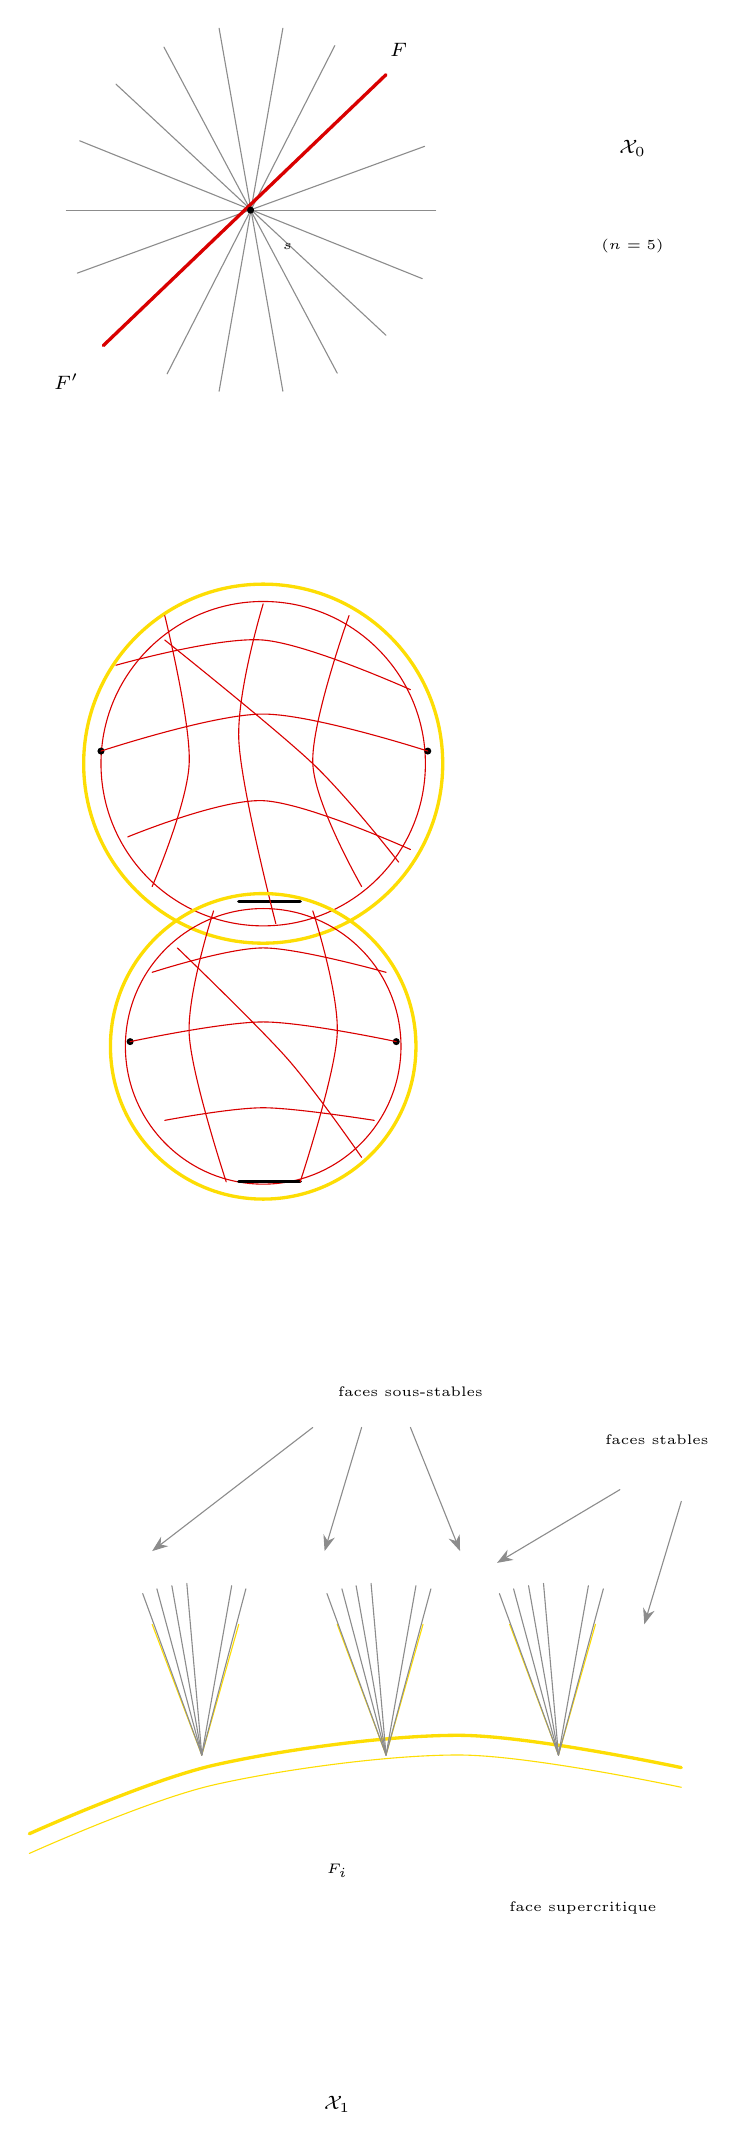
\begin{tikzpicture}[x=1mm,y=1mm,line cap=round,line join=round,font=\scriptsize]
\draw[pencil] (12.5,-26.6) -- (59.4,-26.6);
\draw[pencil] (13.9,-34.6) -- (58,-18.5);
\draw[pencil] (25.3,-47.4) -- (46.6,-5.7);
\draw[pencil] (31.9,-49.6) -- (40,-3.5);
\draw[pencil] (40,-49.6) -- (31.9,-3.5);
\draw[pencil] (46.9,-47.3) -- (24.9,-5.9);
\draw[pencil] (53.1,-42.5) -- (18.8,-10.6);
\draw[pencil] (57.7,-35.3) -- (14.2,-17.8);
\draw[Rd,very thick] (17.2,-43.8) -- (53.1,-9.4);
\node[pt] at (35.9,-26.6) {};
\node[inner sep=1pt] at (54.7,-6.2) {\scriptsize $F$};
\node[inner sep=1pt] at (12.5,-48.4) {\scriptsize $F'$};
\node[inner sep=1pt] at (40.6,-31.2) {\tiny $s$};
\node[inner sep=1pt] at (84.4,-18.8) {\scriptsize $\mathcal{X}_0$};
\node[inner sep=1pt] at (84.4,-31.2) {\tiny $(n=5)$};
\draw[Ye,very thick] (37.5,-96.9) circle[radius=22.8];
\draw[Rd] (37.5,-96.9) circle[radius=20.6];
\node[pt] at (16.9,-95.3) {};
\node[pt] at (58.4,-95.3) {};
\draw[very thick] (34.4,-114.4) -- (42.2,-114.4);
\draw[Rd] plot[smooth, tension=0.55] coordinates {(16.9,-95.3) (37.5,-90.6) (58.4,-95.3)};
\draw[Rd] plot[smooth, tension=0.55] coordinates {(18.8,-84.4) (37.5,-81.2) (56.2,-87.5)};
\draw[Rd] plot[smooth, tension=0.55] coordinates {(20.3,-106.2) (37.5,-101.6) (56.2,-107.8)};
\draw[Rd] plot[smooth, tension=0.55] coordinates {(25,-78.1) (28.1,-96.9) (23.4,-112.5)};
\draw[Rd] plot[smooth, tension=0.55] coordinates {(37.5,-76.6) (34.4,-93.8) (39.1,-117.2)};
\draw[Rd] plot[smooth, tension=0.55] coordinates {(48.4,-78.1) (43.8,-96.9) (50,-112.5)};
\draw[Rd] plot[smooth, tension=0.55] coordinates {(25,-81.2) (43.8,-96.9) (54.7,-109.4)};
\draw[Ye,very thick] (37.5,-132.8) circle[radius=19.4];
\draw[Rd] (37.5,-132.8) circle[radius=17.5];
\node[pt] at (20.6,-132.2) {};
\node[pt] at (54.4,-132.2) {};
\draw[very thick] (34.4,-150) -- (42.2,-150);
\draw[Rd] plot[smooth, tension=0.55] coordinates {(20.6,-132.2) (37.5,-129.7) (54.4,-132.2)};
\draw[Rd] plot[smooth, tension=0.55] coordinates {(23.4,-123.4) (37.5,-120.3) (53.1,-123.4)};
\draw[Rd] plot[smooth, tension=0.55] coordinates {(25,-142.2) (37.5,-140.6) (51.6,-142.2)};
\draw[Rd] plot[smooth, tension=0.55] coordinates {(31.2,-115.6) (28.1,-131.2) (32.8,-150)};
\draw[Rd] plot[smooth, tension=0.55] coordinates {(43.8,-115.6) (46.9,-131.2) (42.2,-150)};
\draw[Rd] plot[smooth, tension=0.55] coordinates {(26.6,-120.3) (40.6,-134.4) (50,-146.9)};
\draw[Ye,very thick] plot[smooth, tension=0.55] coordinates {(7.8,-232.8) (31.2,-224.1) (62.5,-220.3) (90.6,-224.4)};
\draw[Ye] plot[smooth, tension=0.55] coordinates {(7.8,-235.3) (31.2,-226.6) (62.5,-222.8) (90.6,-226.9)};
\draw[Ye] (29.7,-222.8) -- (23.4,-206.2);
\draw[Ye] (29.7,-222.8) -- (34.4,-206.2);
\draw[pencil] (29.7,-222.8) -- (27.8,-201);
\draw[pencil] (29.7,-222.8) -- (25.9,-201.3);
\draw[pencil] (29.7,-222.8) -- (24,-201.7);
\draw[pencil] (29.7,-222.8) -- (22.2,-202.3);
\draw[pencil] (29.7,-222.8) -- (33.5,-201.3);
\draw[pencil] (29.7,-222.8) -- (35.3,-201.7);
\draw[Ye] (53.1,-222.8) -- (46.9,-206.2);
\draw[Ye] (53.1,-222.8) -- (57.8,-206.2);
\draw[pencil] (53.1,-222.8) -- (51.2,-201);
\draw[pencil] (53.1,-222.8) -- (49.3,-201.3);
\draw[pencil] (53.1,-222.8) -- (47.5,-201.7);
\draw[pencil] (53.1,-222.8) -- (45.6,-202.3);
\draw[pencil] (53.1,-222.8) -- (56.9,-201.3);
\draw[pencil] (53.1,-222.8) -- (58.8,-201.7);
\draw[Ye] (75,-222.8) -- (68.8,-206.2);
\draw[Ye] (75,-222.8) -- (79.7,-206.2);
\draw[pencil] (75,-222.8) -- (73.1,-201);
\draw[pencil] (75,-222.8) -- (71.2,-201.3);
\draw[pencil] (75,-222.8) -- (69.3,-201.7);
\draw[pencil] (75,-222.8) -- (67.5,-202.3);
\draw[pencil] (75,-222.8) -- (78.8,-201.3);
\draw[pencil] (75,-222.8) -- (80.7,-201.7);
\node[inner sep=1pt] at (56.2,-176.6) {\tiny faces sous-stables};
\node[inner sep=1pt] at (87.5,-182.8) {\tiny faces stables};
\draw[-{Stealth[length=2mm]},pencil] (43.8,-181.2) -- (23.4,-196.9);
\draw[-{Stealth[length=2mm]},pencil] (50,-181.2) -- (45.3,-196.9);
\draw[-{Stealth[length=2mm]},pencil] (56.2,-181.2) -- (62.5,-196.9);
\draw[-{Stealth[length=2mm]},pencil] (82.8,-189.1) -- (67.2,-198.4);
\draw[-{Stealth[length=2mm]},pencil] (90.6,-190.6) -- (85.9,-206.2);
\node[inner sep=1pt] at (46.9,-237.5) {\tiny $F_i$};
\node[inner sep=1pt] at (78.1,-242.2) {\tiny face supercritique};
\node[inner sep=1pt] at (46.9,-267.2) {\scriptsize $\mathcal{X}_1$};
\end{tikzpicture}
\end{document}
